\documentclass{article}
\usepackage{graphicx} % Required for inserting images
\usepackage{lipsum}
\usepackage[margin=1in, includefoot, includehead]{geometry}
\usepackage{amsmath}
\usepackage{hyperref}
\usepackage{amsfonts}
\usepackage{amssymb}
\usepackage[hidelinks]{hyperref}
\usepackage{fancyhdr}
\usepackage{listings}  % Paquete para insertar código fuente
\usepackage{xcolor}     % Paquete para colores en el código
\lstdefinestyle{python}{
    language=Python,
    basicstyle=\ttfamily\footnotesize, % Tipo de letra
    keywordstyle=\color{blue},         % Color para palabras clave
    commentstyle=\color{gray},         % Color para comentarios
    stringstyle=\color{red},           % Color para strings
    breaklines=true,                    % Romper líneas largas
    frame=single,                       % Marco alrededor del código
    backgroundcolor=\color{gray!10},    % Fondo gris claro
    numbers=left,                       % Numeración de líneas a la izquierda
    numberstyle=\tiny\color{gray}       % Estilo de los números de línea
}
\usepackage[spanish]{babel}
\addto\captionsspanish{\renewcommand{\tablename}{Tabla}}
\pagestyle{fancy}
\fancyhead{}
\fancyfoot{}
\fancyhead[R]{\myTitle}
\fancyfoot[L]{Simulación Numérica}
\fancyfoot[R]{\thepage}
\renewcommand{\footrulewidth}{1pt}
\usepackage[spanish]{babel}
\newcommand{\myTitle}{Informe 1: Examen Parcial}
\newcommand{\myName}{González García, María \\
                    López Rodríguez, Claudia }
\newcommand{\myDate}{\today}

\begin{document}

%PORTADA PRINCIPAL
\begin{titlepage}
    \begin{center}
        
\includegraphics[scale=0.17]{img/UAX.png}\\
        \huge{\textbf{Universidad Alfonso X\\ El Sabio}} \\
        [0.25in] 
        
        \textbf{\Large{Grado en Ingeniería Matemática}}\\
        \Large{Simulación Numérica}\\
    
        \line(1,0){400}\\
        [2mm]
        \textsc{\Large{\myTitle}} \\
        \line(1,0){400} \\
        [1in]
    \end{center}
    \begin{center}
        \textsc{\Large Autor:}	\\
        \myName\\
        [1in]
        \myDate
    \end{center}
\end{titlepage}

%ABSTRACT
\begin{abstract}
En el presente informe se lleva a cabo un análisis detallado de un conjunto de datos experimentales mediante la aplicación de diversos métodos numéricos de interpolación y ajuste. Se implementan polinomios de interpolación de Lagrange y Splines Cúbicos, así como ajustes por regresión lineal y no lineal, considerando modelos polinómicos de distintos grados y funciones exponenciales. Para ello, se desarrollan algoritmos en Python que permiten realizar estos cálculos de manera eficiente y precisa. Finalmente, se presentan y discuten los resultados obtenidos, evaluando la precisión y aplicabilidad de cada método en el contexto de la simulación numérica.
\end{abstract}


%ÍNDICE
\newpage
\tableofcontents

%INTRODUCCIÓN
\newpage
\section{Introducción.}
El examen consistirá en hacer un análisis de datos experimentales. Cada grupo tendrá que elegir uno de los 6 archivos que se encuentran en la plataforma, denominados \texttt{Datos Grupos N.txt}, dónde $N$ representa el número del grupo.

Con los datos dados en el archivo, los integrantes tendrán que realizar los siguientes ajustes:

\begin{enumerate}
    \item Desarrollar una función en Python que determine el polinomio de interpolación de Lagrange que se ajuste a los datos entregados.
    \item Desarrollar una función en Python que determine los polinomios de interpolación mediante Splines Cúbicos.
    \item Ajustar los datos entregados mediante regresión lineal a polinomios de grado $1$, $2$, $3$ y $4$, y a la función $y = a_0 x^{a_1}$ haciendo una transformación de los datos.
    \item Ajustar los datos entregados mediante regresi\'on no lineal a las siguientes funciones:
    \begin{enumerate}
        \item $f(x) = a_0 - a_1 e^{-a_2 x}$
        \item $f(x) = a_0 x - a_1 e^{-a_2 x}$
        \item $f(x) = a_0 x^2 - a_1 e^{-a_2 x}$
    \end{enumerate}
\end{enumerate}
\vspace{8mm}
\noindent \textbf{En virtud de que nuestro estudio se enmarca dentro del Grupo 2, se procederá a emplear el archivo: \texttt{Datos Grupo 2.txt}.} Seguidamente, se presenta una representación gráfica de los datos originales (véase la Figura~\ref{fig:datosoriginales}).  

\begin{figure}[h]  
    \centering  
    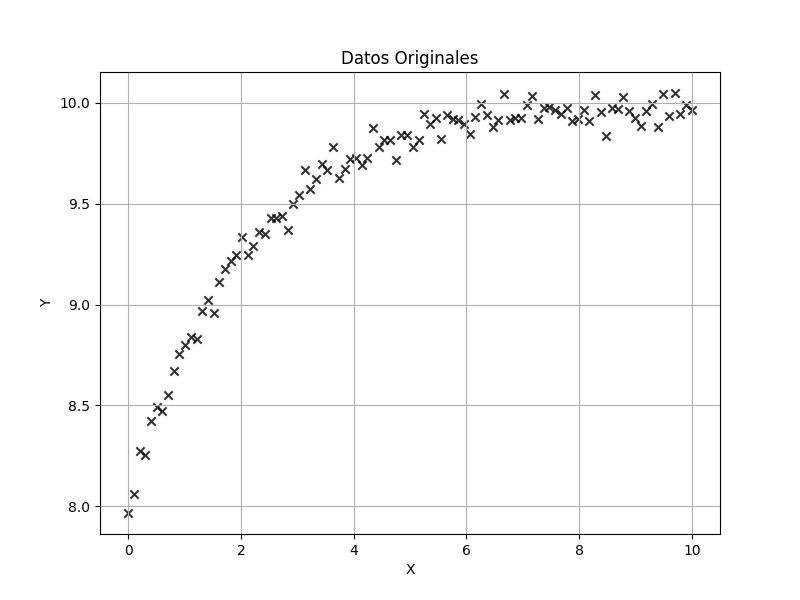
\includegraphics[width=0.6\linewidth]{img/datos.png}  
    \caption{Distribución de los datos del archivo.}
    \label{fig:datosoriginales}  
\end{figure}  


%MÉTODOS Y MODELOS MATEMÁTICOS
\newpage
\section{Métodos y modelos matemáticos.}
\subsection{Interpolación.}
\subsubsection{Interpolación de Newton.}
\label{subsec:newton}
La \textbf{interpolación de Newton} es un método numérico utilizado para encontrar un polinomio que pase exactamente por un conjunto de puntos dados. Este método se basa en la construcción de un \textbf{polinomio de diferencias divididas}, lo que permite una formulación fácil de actualizar cuando se agregan nuevos puntos.

\noindent \textbf{Definición del Polinomio de Newton.}
Dado un conjunto de $n+1$ puntos distintos $(x_0, y_0), (x_1, y_1), \dots, (x_n, y_n)$, el polinomio interpolador de Newton se define como:

\begin{equation}
f_n(x) = f[x_0] + f[x_0, x_1](x - x_0) + f[x_0, x_1, x_2](x - x_0)(x - x_1) + \dots + f[x_0, x_1, \dots, x_n] \prod_{i=0}^{n-1} (x - x_i).
\end{equation}

\noindent \textbf{Diferencias divididas.}  
Los coeficientes del polinomio se calculan mediante \textbf{diferencias divididas}, las cuales se definen recursivamente de la siguiente manera:

\begin{equation}
f[x_i, x_{i+1}, \dots, x_{i+k}] = \frac{f[x_{i+1}, \dots, x_{i+k}] - f[x_i, \dots, x_{i+k-1}]}{x_{i+k} - x_i}.
\end{equation}

Este enfoque permite que el cálculo del polinomio sea altamente eficiente, ya que cada diferencia dividida de orden superior se construye a partir de diferencias divididas de orden inferior, lo que reduce significativamente el costo computacional. La Figura \ref{fig:diferencias-div} ilustra la estructura recursiva del cálculo de diferencias divididas, dónde cada término de orden superior depende de los términos de orden inferior.

\begin{figure}[h]
    \centering
    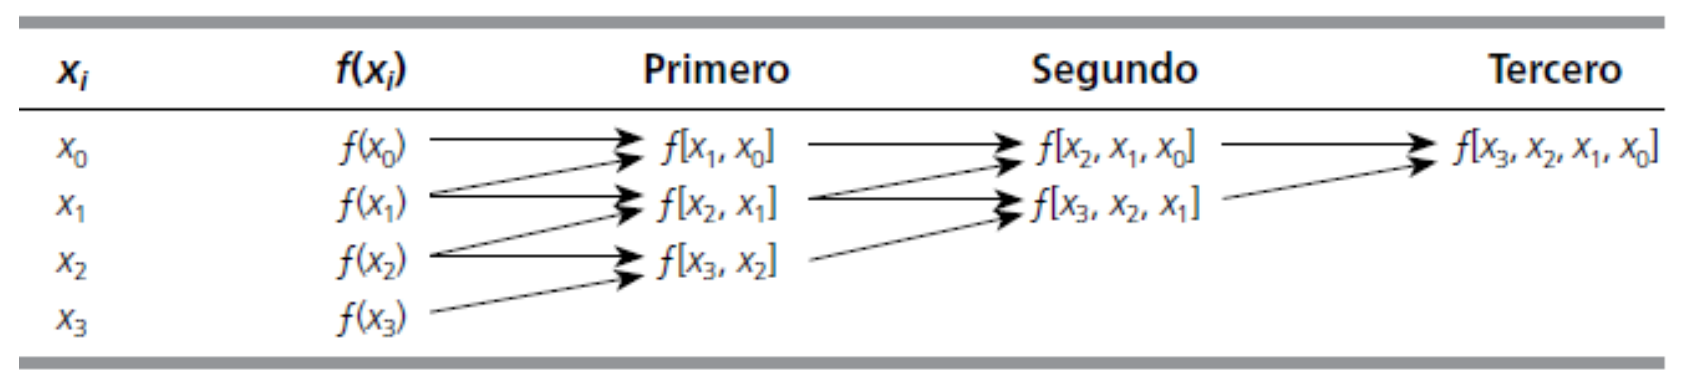
\includegraphics[width=0.7\linewidth]{img/diferencias-div.png}
    \caption{Representación gráfica de la naturaleza recursiva de las diferencias divididas finitas.}
    \label{fig:diferencias-div}
\end{figure}

Dado que la construcción del polinomio de Newton es incremental, es posible construir $f_n(x)$ a partir de $f_{n-1}(x)$, lo que hace que este método sea eficiente para cálculos iterativos. Esto es particularmente útil cuando se agregan nuevos datos al conjunto original, ya que no es necesario recalcular completamente el polinomio, sino únicamente actualizar los términos adicionales.\\

\noindent \textbf{Error de la Interpolación de Newton.}
El error de interpolación de Newton nos permite estimar qué tan precisa es la aproximación del polinomio interpolador respecto a la función original. La fórmula del error se expresa como:

\begin{equation}
R_n(x) = f[x_0, x_1, \dots, x_n, x] \prod_{i=0}^{n} (x - x_i).
\end{equation}

Si asumimos que la función $f(x)$ es $n+1$ veces derivable en un intervalo que contiene los puntos $x_0, x_1, \dots, x_n$, el término de error puede expresarse en términos de la derivada de orden $n+1$:

\begin{equation}
R_n(x) = \frac{f^{(n+1)}(\xi)}{(n+1)!} \prod_{i=0}^{n} (x - x_i), \quad \text{dónde } \xi \in [x_0, x_n].
\end{equation}


\subsubsection{Interpolación de Lagrange.}
\label{subsec:lagrange}
La \textbf{interpolación de Lagrange} es un método numérico utilizado para encontrar un polinomio de grado $n$ que pasa exactamente por un conjunto de $n+1$ puntos dados \cite{lagrange1, lagrange2}. Este método se basa en la construcción de una combinación lineal de \textbf{polinomios base de Lagrange}, evitando la necesidad de calcular diferencias divididas, como en la interpolación de Newton.\\

\noindent \textbf{Definición del Polinomio de Lagrange.}  
Dado un conjunto de $n+1$ puntos distintos $(x_0, y_0), (x_1, y_1), \dots, (x_n, y_n)$, el polinomio interpolador de Lagrange se define como \cite{lagrange3}:
\begin{equation}
f_n(x) = \sum_{i=0}^{n} f(x_i) L_i(x),
\end{equation}
dónde los \textbf{polinomios base de Lagrange} $L_i(x)$ están dados por:
\begin{equation}
L_i(x) = \prod_{\substack{j=0 \\ j\neq i}}^n \frac{x - x_j}{x_i - x_j}.
\end{equation}

Cada $L_i(x)$ es un polinomio de grado  $n$ que toma el valor de 1 en $x_i$ y 0 en los demás puntos del conjunto. Esto garantiza que el polinomio interpolador $f_n(x)$ pase exactamente por los valores $f(x_i)$.\\

\noindent \textbf{Propiedades del Polinomio de Lagrange.} El método de interpolación de Lagrange tiene varias características importantes:

\begin{itemize}
    \item \textbf{Evita el cálculo de diferencias divididas}, lo que facilita su implementación computacional.
    \item \textbf{Los puntos de interpolación pueden estar en cualquier orden} y no necesitan ser equidistantes.
    \item Es un método \textbf{global}, ya que cualquier modificación en un solo punto afecta a todo el polinomio interpolador.
    \item Para cada nuevo punto agregado, es necesario recalcular todos los polinomios base $ L_i(x) $.
\end{itemize}

Su principal desventaja es su inestabilidad para valores grandes de $n$, lo que puede generar oscilaciones no deseadas en la función interpolante \cite{lagrange1}. En casos dónde se requiera mayor estabilidad, se recomienda utilizar métodos alternativos como los \textbf{Splines Cúbicos} (véase Sección~\ref{subsec:splines-cubicos}).


\newpage
\subsubsection{Interpolación por Splines Cúbicos}
\label{subsec:splines-cubicos}

La \textbf{interpolación por Splines Cúbicos} es un método numérico utilizado para aproximar una función mediante polinomios de tercer grado (\textit{Splines Cúbicos}) en cada subintervalo del dominio \cite{splines1, splines2}.
A diferencia de la interpolación polinómica global, los Splines Cúbicos garantizan una mayor estabilidad y suavidad, evitando oscilaciones extremas en los extremos del intervalo.\\

\noindent \textbf{Definición del Spline Cúbico.}  
Dado un conjunto de $n+1$ puntos $(x_0, y_0), (x_1, y_1), \dots, (x_n, y_n)$, se define un conjunto de polinomios cúbicos $S_i(x)$ para cada subintervalo $[x_i, x_{i+1}]$ \cite{splines3}:
\begin{equation}
S_i(x) = a_i + b_i (x - x_i) + c_i (x - x_i)^2 + d_i (x - x_i)^3, \quad \text{para } x \in [x_i, x_{i+1}].
\end{equation}
Estos polinomios se construyen de manera que se garantice la \textbf{continuidad} de la función interpoladora y sus derivadas hasta el orden 2 \cite{splines4}.

\noindent \textbf{Condiciones de continuidad.} Para garantizar que la interpolación por Splines Cúbicos sea suave y precisa, se deben cumplir las siguientes condiciones:
\begin{itemize}
    \item \textbf{Condición de interpolación}: Cada spline pasa exactamente por los puntos de datos:
    $$S_i(x_i) = y_i, \quad S_i(x_{i+1}) = y_{i+1}.$$    
    \item \textbf{Continuidad de la primera derivada}: Las derivadas de primer orden deben ser continuas en los puntos de unión:
    $$ S_i'(x_{i+1}) = S_{i+1}'(x_{i+1}). $$

    \item \textbf{Continuidad de la segunda derivada}: Las derivadas de segundo orden también deben ser continuas:
    $$S_i''(x_{i+1}) = S_{i+1}''(x_{i+1}).$$

    \item \textbf{Condición de contorno}: Para definir un conjunto único de Splines Cúbicos, se requieren condiciones adicionales en los extremos:
    $$
        S_0''(x_0) = 0, \quad S_{n-1}''(x_n) = 0
    $$
\end{itemize}

\noindent \textbf{Construcción del sistema de ecuaciones.}  Para determinar los coeficientes $a_i, b_i, c_i, d_i$, se debe resolver un sistema de ecuaciones que garantice la continuidad de la primera y segunda derivada en cada subintervalo. La clave en la construcción de los Splines Cúbicos es calcular las \textbf{segundas derivadas} $M_i = S_i''(x_i)$ en cada nodo. 

\textbf{Planteamiento del sistema de ecuaciones. } Dado un conjunto de $n+1$ puntos de interpolación $(x_0, y_0), (x_1, y_1), \dots, (x_n, y_n)$, el sistema de ecuaciones se expresa como:

\begin{equation}
    h_{i-1} M_{i-1} + 2(h_{i-1} + h_i) M_i + h_i M_{i+1} = 6 \left( \frac{y_{i+1} - y_i}{h_i} - \frac{y_i - y_{i-1}}{h_{i-1}} \right),
\end{equation}
dónde $h_i = x_{i+1} - x_i$ representa la distancia entre nodos consecutivos.

Este sistema se puede expresar en forma matricial como:

\[
\begin{bmatrix}
    2(h_0 + h_1) & h_1 & 0 & \dots & 0 \\
    h_1 & 2(h_1 + h_2) & h_2 & \dots & 0 \\
    0 & h_2 & 2(h_2 + h_3) & \dots & 0 \\
    \vdots & \vdots & \vdots & \ddots & h_{n-2} \\
    0 & 0 & 0 & h_{n-2} & 2(h_{n-2} + h_{n-1})
\end{bmatrix}
\begin{bmatrix}
    M_1 \\
    M_2 \\
    M_3 \\
    \vdots \\
    M_{n-1}
\end{bmatrix}
=
\begin{bmatrix}
    6 \left( \frac{y_2 - y_1}{h_1} - \frac{y_1 - y_0}{h_0} \right) \\
    6 \left( \frac{y_3 - y_2}{h_2} - \frac{y_2 - y_1}{h_1} \right) \\
    6 \left( \frac{y_4 - y_3}{h_3} - \frac{y_3 - y_2}{h_2} \right) \\
    \vdots \\
    6 \left( \frac{y_n - y_{n-1}}{h_{n-1}} - \frac{y_{n-1} - y_{n-2}}{h_{n-2}} \right)
\end{bmatrix}
\]

\textbf{Resolución del sistema de ecuaciones.} Una vez resueltas las segundas derivadas $M_i$, los coeficientes del Spline Cúbico se obtienen mediante:

$$
\begin{cases}
    a_i = y_i, \\
    b_i = \frac{y_{i+1} - y_i}{h_i} - \frac{h_i}{6} (2M_i + M_{i+1}), \\
    c_i = \frac{M_i}{2}, \\
    d_i = \frac{M_{i+1} - M_i}{6h_i}.
\end{cases}
$$

\vspace{5mm}
\noindent \textbf{Propiedades de los Splines Cúbicos.} Los Splines Cúbicos presentan varias ventajas sobre la interpolación polinómica global \cite{splines1, splines3}.

\begin{itemize}
    \item \textbf{Mayor estabilidad numérica}: Al ser polinomios de grado bajo en cada subintervalo, se evitan las oscilaciones extremas presentes en la interpolación de Lagrange o Newton.
    \item \textbf{Mayor precisión}: Se ajustan mejor a funciones con cambios de curvatura sin necesidad de polinomios de grado elevado.
    \item \textbf{Continuidad garantizada}: Las derivadas hasta el segundo orden son continuas, proporcionando una transición suave entre intervalos.
\end{itemize}

\newpage
\subsection{Regresión por mínimos cuadrados.}
Un problema al hacer ajustes de curvas, viene dado cuándo los datos tienen errores sustanciales. De este modo, es posible que una interpolación de datos intermedios no sea apropiada. Una forma de hacerlo es obtener una curva que minimice la discrepancia entre los puntos y la curva, esto se denomina \textbf{regresión por mínimos cuadrados}.

\subsubsection{Regresión Lineal.}
\label{subsec:regresionlineal}
La \textbf{regresión lineal} busca modelar la relación entre una variable dependiente $y$ y una variable independiente $x$ mediante una ecuación de primer grado \cite{polinomico1, polinomico2}.

\begin{equation}
    y = a_0 + a_1 x + \varepsilon.
\end{equation}
dónde:
\begin{itemize}
    \item $a_0$ es la ordenada al origen.
    \item $a_1$ es la pendiente de la recta, que indica cómo varía $y$ con respecto a $x$.
    \item $\varepsilon$ es el error asociado a cada observación.
\end{itemize}
El objetivo del modelo es encontrar los valores de $a_0$ y $a_1$ que minimicen la \textbf{suma de los errores cuadráticos}, definida como:
$$
    S_r = \sum_{i=1}^{n} (y_i - \hat{y}_i)^2 = \sum_{i=1}^{n} (y_i - a_0 - a_1x_i)^2 .
$$

\noindent \textbf{Estimación de los coeficientes.}
Los coeficientes $a_0$ y $a_1$ se determinan mediante el \textbf{método de mínimos cuadrados} \cite{polinomico3}. Se deriva la suma de los errores cuadráticos con respecto a estos coeficientes y se iguala a cero:
\begin{equation}
    S_r = \sum_{i=1}^{n} (y_i - a_0 - a_1x_i)^2.
\end{equation}
Derivando con respecto a $a_0$ y $a_1$, obtenemos el siguiente sistema de ecuaciones normales:
\begin{equation}
\begin{cases}
    n a_0 + a_1 \sum x_i = \sum y_i, \\
    a_0 \sum x_i + a_1 \sum x_i^2 = \sum x_i y_i.
\end{cases}
\end{equation}
Este sistema de ecuaciones se puede expresar en forma matricial como:
\[
\begin{bmatrix}
    n & \sum x_i \\
    \sum x_i & \sum x_i^2
\end{bmatrix}
\begin{bmatrix}
    a_0 \\ a_1
\end{bmatrix}
=
\begin{bmatrix}
    \sum y_i \\ \sum x_i y_i
\end{bmatrix}.
\]
Si despejamos los coeficientes del sistema de ecuaciones normales, obtenemos las siguientes expresiones:
$$
\begin{cases}
    a_1 = \frac{n \sum x_i y_i - \sum x_i \sum y_i}{n \sum x_i^2 - (\sum x_i)^2},\\
    a_0 = \bar{y} - a_1 \bar{x}
\end{cases}
$$
Este sistema garantiza que la recta encontrada minimiza la suma de los errores al cuadrado.\\

\noindent\textbf{Errores de la Regresión Lineal.}
\begin{enumerate}
    \item \textbf{Error de la Regresión Lineal.}
    $$
    S_r = \sum_{i=1}^{n} e_i^2 = \sum_{i=1}^{n} (y_i - a_0 - a_1 x_i)^2
    $$
    \item \textbf{Error Estándar de Estimación.} La desviación estándar y esta medida miden ambas la dispersión. Sin embargo, la diferencia notoria es que la desviación estándar mide la dispersión de los valores $y$ con respecto a su media (sin considerar $x$),  mientras que el \textbf{error estándar} de estimación mide la dispersión de los valores $y$ con respecto a la recta de regresión (considerando $x$).
    $$
    S_{y/x} = \sqrt{\frac{S_r}{n-2}}
    $$
\end{enumerate}

\noindent \textbf{Coeficiente de Determinación: $r^2$.}
Para evaluar la calidad del ajuste, se utiliza el \textbf{coeficiente de determinación} $R^2$, que mide la proporción de variabilidad en $y$ explicada por el modelo \cite{polinomico4}.
\begin{equation}
    r^2 = \frac{S_t -S_r}{S_t} \quad \text{ siendo } S_t \text{ la desviación  estándar para los datos } y_i.
\end{equation}
El coeficiente $r^2$ toma valores entre 0 y 1:
\begin{itemize}
    \item $r^2 = 1$ indica que el modelo explica el 100\% de la variabilidad de $y$.
    \item $r^2 = 0$ indica que el modelo no explica nada de la variabilidad de $ y $.
\end{itemize}
\noindent \textbf{Coeficiente de Correlación: $r$.} Es simplemente la raíz del coeficiente de determinación, cuánto más se aproxime el valor a 1, mejor es
el ajuste.
\begin{equation}
    r = \sqrt{\frac{S_t -S_r}{S_t}} \quad \text{ siendo } S_t \text{ la desviación  estándar para los datos } y_i.
\end{equation}

\noindent\textbf{Limitaciones de la Regresión Lineal.} Aunque la regresión lineal es una técnica poderosa, presenta algunas limitaciones:

\begin{itemize}
    \item \textbf{No captura relaciones no lineales} entre las variables.
    \item Es sensible a \textbf{valores atípicos}, los cuales pueden afectar significativamente la estimación de los coeficientes.
    \item Supone que los errores son independientes y tienen varianza constante.
\end{itemize}

Cuando estas condiciones no se cumplen, pueden ser necesarios otros modelos como la regresión polinomial (véase Sección~\ref{subsec:rpolinomial}) o regresión no lineal (véase Sección~\ref{subsec:rnolineal}).

\newpage
\subsubsection{Regresión Polinomial.}
\label{subsec:rpolinomial}
La \textbf{regresión polinomial} es una extensión de la regresión lineal que permite ajustar modelos más flexibles cuando la relación entre las variables no es lineal \cite{polinomico1, polinomico5}. En lugar de una línea recta, se ajusta un polinomio de grado $n$ a los datos.\\

\noindent \textbf{Modelo de regresión polinomial.}  
El modelo matemático para una regresión polinomial de grado $n$ es:
\begin{equation}
    y = a_0 + a_1 x + a_2 x^2 + \dots + a_n x^n + \varepsilon,
\end{equation}
dónde:
\begin{itemize}
    \item $y$ es la variable dependiente, $x$ es la variable independiente y $\varepsilon$ es el término de error.
    \item $a_0, a_1, \dots, a_n$ son los coeficientes del polinomio.
\end{itemize}

\noindent \textbf{Método de Mínimos Cuadrados.} Para determinar los coeficientes $a_0, a_1, \dots, a_n$, se utiliza el \textbf{método de mínimos cuadrados}, similar a la regresión lineal \cite{polinomico2}.
$$
    \sum_{i=1}^{n} y_i = a_0 \sum_{i=1}^{n} 1 + a_1 \sum_{i=1}^{n} x_i + a_2 \sum_{i=1}^{n} x_i^2 + \dots + a_n \sum_{i=1}^{n} x_i^n.
$$
Este sistema se resuelve generalmente mediante álgebra matricial:

\[
\begin{bmatrix}
    n & \sum x_i & \sum x_i^2 & \dots & \sum x_i^n \\
    \sum x_i & \sum x_i^2 & \sum x_i^3 & \dots & \sum x_i^{n+1} \\
    \sum x_i^2 & \sum x_i^3 & \sum x_i^4 & \dots & \sum x_i^{n+2} \\
    \vdots & \vdots & \vdots & \ddots & \vdots \\
    \sum x_i^n & \sum x_i^{n+1} & \sum x_i^{n+2} & \dots & \sum x_i^{2n}
\end{bmatrix}
\begin{bmatrix}
    a_0 \\ a_1 \\ a_2 \\ \vdots \\ a_n
\end{bmatrix}
=
\begin{bmatrix}
    \sum y_i \\ \sum x_i y_i \\ \sum x_i^2 y_i \\ \vdots \\ \sum x_i^n y_i
\end{bmatrix}
\]
\vspace{4mm}

\noindent \textbf{Elección del Grado del Polinomio.} Uno de los aspectos clave de la regresión polinomial es la elección del grado $n$. Si $n$ es muy bajo, el modelo puede ser demasiado simple y no capturar correctamente la tendencia de los datos (\textbf{subajuste}). Si $n$ es demasiado alto, el modelo puede ajustarse demasiado a los datos de entrenamiento y perder capacidad de generalización (\textbf{sobreajuste}).

En la práctica, \textbf{el grado del polinomio se elige analizando el error de estimación} y validando el modelo con datos adicionales \cite{polinomico4}.\\

\noindent \textbf{Error estándar de estimación.} En el caso de la \textbf{regresión polinomial}, el error estándar de estimación $s_{y/x}$ mide la dispersión de los valores observados $y_i$ en torno a la curva ajustada del polinomio. Se calcula como:
\begin{equation}
    s_{y/x} = \sqrt{\frac{S_r}{n - (m + 1)}}
\end{equation}
dónde:
\begin{itemize}
    \item $n$ es el número total de observaciones en el conjunto de datos.
    \item $m$ es el \textbf{grado del polinomio} ajustado.
\end{itemize}

\newpage
\subsubsection{Regresión Lineal Múltiple.}
La \textbf{regresión lineal múltiple} es una extensión de la regresión lineal simple (véase Sección~\ref{subsec:regresionlineal}) que permite modelar la relación entre una variable dependiente $y$ y múltiples variables independientes (\cite{polinomico3}) $x_1, x_2, \dots, x_m$. Se utiliza cuando la variable de interés depende de más de un factor.\\

\noindent \textbf{Modelo de regresión lineal múltiple.}  
El modelo matemático se expresa como:
\begin{equation}
    y = a_0 + a_1 x_1 + a_2 x_2 + \dots + a_m x_m + \varepsilon,
\end{equation}
\vspace{2mm}

\noindent \textbf{Estimación de los coeficientes mediante Mínimos Cuadrados.} Al igual que en la regresión lineal simple, los coeficientes $a_0, a_1, \dots, a_m$ se determinan minimizando la suma de los errores cuadráticos. El sistema de ecuaciones normal asociado se expresa en forma matricial como:
\[
\begin{bmatrix}
    n & \sum x_{1i} & \sum x_{2i} & \dots & \sum x_{mi} \\
    \sum x_{1i} & \sum x_{1i}^2 & \sum x_{1i} x_{2i} & \dots & \sum x_{1i} x_{mi} \\
    \sum x_{2i} & \sum x_{1i} x_{2i} & \sum x_{2i}^2 & \dots & \sum x_{2i} x_{mi} \\
    \vdots & \vdots & \vdots & \ddots & \vdots \\
    \sum x_{mi} & \sum x_{1i} x_{mi} & \sum x_{2i} x_{mi} & \dots & \sum x_{mi}^2
\end{bmatrix}
\begin{bmatrix}
    a_0 \\ a_1 \\ a_2 \\ \vdots \\ a_m
\end{bmatrix}
=
\begin{bmatrix}
    \sum y_i \\ \sum x_{1i} y_i \\ \sum x_{2i} y_i \\ \vdots \\ \sum x_{mi} y_i
\end{bmatrix}
\]
Este sistema se resuelve utilizando álgebra matricial mediante la inversa de la matriz de coeficientes \cite{polinomico5}.
\begin{equation}
    A = (X^T X)^{-1} X^T Y,
\end{equation}
dónde:
\begin{itemize}
    \item $X$ es la matriz de datos de tamaño $n \times (m+1)$.
    \item $Y$ es el vector de valores observados de $y$.
    \item $A$ es el vector de coeficientes $(a_0, a_1, \dots, a_m)$.
\end{itemize}

\noindent \textbf{Suposiciones de la Regresión Lineal Múltiple.} Para que la regresión lineal múltiple sea válida, deben cumplirse las siguientes condiciones \cite{polinomico2}.

\begin{itemize}
    \item Linealidad: La relación entre las variables es aproximadamente lineal.
    \item Independencia: No debe haber correlación entre los residuos.
    \item Homoscedasticidad: La varianza de los errores debe ser constante.
    \item No colinealidad: Las variables predictoras no deben estar altamente correlacionadas entre sí.
    \item Distribución normal de los errores: Los residuos deben seguir una distribución normal.
\end{itemize}

\noindent \textbf{Error estándar de estimación.} El \textbf{error estándar de estimación} $s_{y/x}$ mide la dispersión de los valores observados $y_i$ en torno a la hiperplano de regresión. Se define como:
\begin{equation}
    s_{y/x} = \sqrt{\frac{S_r}{n - (m+1)}}
\end{equation}

\begin{itemize}
    \item Si $s_{y/x}$ es pequeño, los valores predichos $\hat{y}_i$ están cerca de los valores observados $y_i$, lo que indica un buen ajuste del modelo.
    \item Si $s_{y/x}$ es grande, la dispersión es alta, lo que sugiere que el modelo no explica bien la variabilidad de los datos.
\end{itemize}

\newpage
\subsubsection{Regresión No Lineal.}
\label{subsec:rnolineal}
La \textbf{regresión no lineal} es un método estadístico que permite ajustar un modelo matemático cuando la relación entre las variables dependiente $y$ e independientes $x$ no es lineal en los parámetros \cite{nolineal1, nolineal2}. Esto significa que no se puede expresar como una combinación lineal de los coeficientes a estimar. Su forma general es:
\begin{equation}
    y = f(x, a_0, a_1, \dots, a_m) + \varepsilon,
\end{equation}
dónde $f(x, a_0, a_1, \dots, a_m)$ es una función no lineal en los coeficientes $a_i$, y $\varepsilon$ es el término de error.

A diferencia de la regresión lineal, en la regresión no lineal \textbf{no se pueden obtener soluciones exactas mediante ecuaciones normales}, por lo que se emplean métodos iterativos para minimizar la suma de los errores cuadráticos \cite{nolineal1}.
$S = \sum_{i=1}^{n} (y_i - f(x_i, a_0, a_1, \dots, a_m))^2.$
\vspace{3mm}

\noindent \textbf{Aproximación mediante Serie de Taylor.} Para resolver este problema, una técnica común es \textbf{linealizar el modelo} usando una \textbf{expansión en serie de Taylor} alrededor de los valores actuales de los coeficientes (\cite{nolineal2}) $a_m^{(j)}$:

\begin{equation}
    f(x, a_m^{(j+1)}) \approx f(x, a_m^{(j)}) + \sum_{k=0}^{m} \frac{\partial f}{\partial a_k} \Delta a_k.
\end{equation}

Aquí, $\Delta a_k$ representa el cambio en los coeficientes en la iteración $j+1$. Esta aproximación convierte el problema no lineal en un \textbf{sistema de ecuaciones lineales}.\\

\noindent \textbf{Resolución mediante Mínimos Cuadrados No Lineales.} Al reformular el problema en términos matriciales, se obtiene (\cite{nolineal1}).

\begin{equation}
    \mathbf{Z_J} \mathbf{\Delta A} = \mathbf{D},
\end{equation}
dónde:
\begin{itemize}
    \item $\mathbf{Z_J}$ es la \textbf{matriz Jacobiana}, con elementos:
    $
        {Z_J}_{ik} = \frac{\partial f}{\partial a_k} \bigg|_{(x_i, a_k^{(j)})}.
    $

    \item $\mathbf{D}$ es el \textbf{vector de residuos}, dado por:
    $
        d_i = y_i - f(x_i, a_0, a_1, \dots, a_m).
    $

    \item $\mathbf{\Delta A}$ es el vector de corrección de los coeficientes, que se obtiene resolviendo:

    \begin{equation}
        \mathbf{\Delta A} = (\mathbf{Z_J}^T \mathbf{Z_J})^{-1} \mathbf{Z_J}^T \mathbf{D}.
    \end{equation}
\end{itemize}
Este sistema permite encontrar $\Delta A$, que se usa para actualizar los parámetros:

\begin{equation}
    a_m^{(j+1)} = a_m^{(j)} + \Delta a_m.
\end{equation}

\noindent \textbf{Método Iterativo hasta la Convergencia.} El procedimiento para resolver la regresión no lineal mediante mínimos cuadrados sigue los siguientes pasos (\cite{nolineal2}):

\begin{enumerate}
    \item Se eligen valores iniciales para los coeficientes $a_0, a_1, \dots, a_m$.
    \item Se evalúan los valores predichos $f(x_i, a_m^{(j)})$ y la matriz Jacobiana $\mathbf{Z_J}$.
    \item Se calcula $\mathbf{\Delta A}$ resolviendo $\mathbf{Z_J}^T \mathbf{Z_J} \mathbf{\Delta A} = \mathbf{Z_J}^T \mathbf{D}$.
    \item Se actualizan los coeficientes con $a_m^{(j+1)} = a_m^{(j)} + \Delta a_m$.
    \item Se repite el proceso hasta que la variación de los coeficientes sea menor que un umbral de tolerancia $\varepsilon$.
\end{enumerate}

\newpage
\subsubsection{Linealización de Relaciones No Lineales.}
\label{subsec:linealizacion}
Cuando un modelo no es lineal en sus parámetros, es posible aplicar transformaciones matemáticas para convertirlo en una forma lineal. Este proceso se conoce como \textbf{linealización} y permite resolver el problema utilizando el método de mínimos cuadrados de la regresión lineal. A continuación, se presentan algunos modelos no lineales comunes y su transformación.

\noindent \textbf{Transformación de Modelos No Lineales.}
\begin{itemize}
    \item \textbf{Modelo Exponencial.} Se utiliza para representar crecimiento o decaimiento exponencial. Su forma general es:
    \begin{equation}
        y = a_0 - a_1 e^{-a_2 x}.
    \end{equation}
    Para linealizar este modelo, tomamos el logaritmo natural en ambos lados:
    $$\ln(-(y - a_0)) = \ln a_1 - a_2 x.$$
    Esto permite reescribir la ecuación en forma lineal $Y = A + BX$, dónde:
    \begin{equation}
        Y = \ln(-(y - a_0)), \quad A = \ln a_1, \quad B = -a_2, \quad X = x.
    \end{equation}
    Luego, se aplica regresión lineal sobre $Y$ y $X$ para estimar $A$ y $B$, y finalmente recuperar $a_1$ y $a_2$.

    \item \textbf{Modelo de Potencia.} Se usa cuando la relación entre $y$ y $x$ sigue una ley de potencia:
    \begin{equation}
        y = a_0 x^{a_1}.
    \end{equation}
    Aplicando logaritmos:
    $$\ln y = \ln a_0 + a_1 \ln x.$$
    Esto permite usar regresión lineal para encontrar $\ln a_0$ y $a_1$, y luego recuperar $a_0$ mediante la exponencial.

    \item \textbf{Modelo Hiperbólico.} Se emplea para representar relaciones inversas:
    \begin{equation}
        y = \frac{a_0}{a_1 + x}
    \end{equation}
    Tomamos el recíproco:
    $$
        \frac{1}{y} = \frac{x}{a_0} + \frac{a_1}{a_0} .
    $$
    Ahora, la relación es lineal, lo que permite estimar los parámetros mediante regresión lineal.
\end{itemize}

\noindent \textbf{Resolución Mediante Mínimos Cuadrados.} Una vez que los modelos han sido transformados en expresiones lineales, se pueden resolver usando \textbf{métodos de regresión lineal} (véase Sección~\ref{subsec:regresionlineal}).\\

\noindent \textbf{Síntesis.} La linealización de modelos no lineales permite utilizar técnicas de regresión lineal para estimar los parámetros de modelos complejos. Sin embargo, las transformaciones pueden afectar la distribución del error y deben aplicarse con cuidado. En casos dónde la linealización no es viable, se recomienda utilizar métodos de ajuste no lineales como el \textbf{método de Levenberg-Marquardt}.


%RESULTADOS
\newpage
\section{Resultados.}
\subsection{Ejercicio 1: Interpolación de Lagrange.}
\label{subsec:rlagrange}
Se implementó la interpolación de Lagrange sobre el conjunto de datos experimentales, obteniéndose un polinomio interpolador que pasa exactamente por los puntos originales. La interpolación se evaluó en un conjunto de 100 puntos dentro del intervalo de análisis, generando la siguiente gráfica (véase la Figura~\ref{fig:lagrange}) :

\begin{figure}[h]
    \centering
    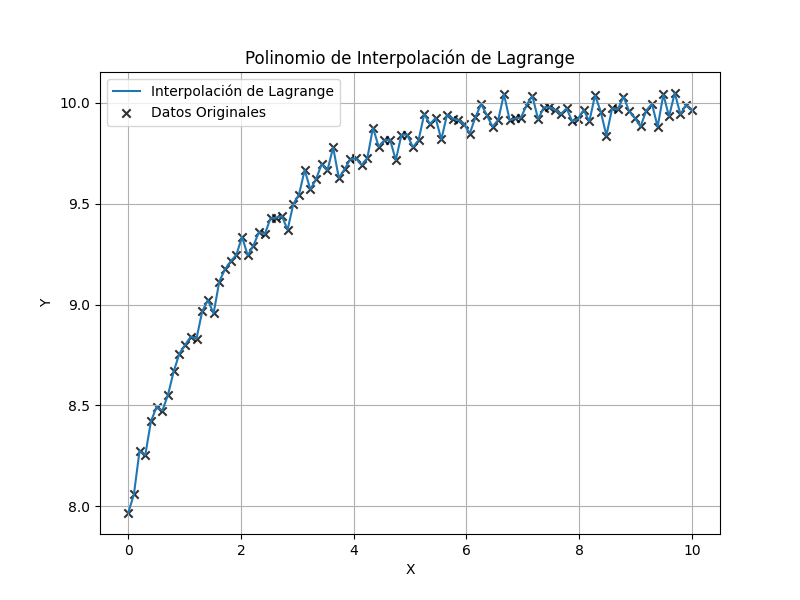
\includegraphics[width=0.6\linewidth]{img/polinomio lagrange.png}
    \caption{Interpolación de Lagrange aplicada a los datos experimentales.}
    \label{fig:lagrange}
\end{figure}

Los resultados muestran que el polinomio ajusta con precisión los datos originales, reproduciendo exactamente los valores en los nodos dados. Para analizar con mayor detalle el comportamiento de la interpolación, se han identificado tres regiones dentro del intervalo (véase la Figura~\ref{fig:lagrangeintervalos}) :

\begin{figure}[h]
    \centering
    
\includegraphics[width=0.9\linewidth]{img/lagrange_secciones.png}
    \caption{Análisis por Regiones de la Interpolación de Lagrange.}
    \label{fig:lagrangeintervalos}
\end{figure}
\begin{itemize}
    \item \textbf{Región 1: $x \in [0,3]$.}  
    En esta zona, el polinomio de interpolación de Lagrange es una \textbf{aproximación adecuada}, ya que respeta la forma funcional de los datos sin introducir desviaciones artificiales. La función interpolada presenta continuidad y suavidad, reflejando fielmente la tendencia creciente de los datos por la distribución homogénea de los puntos. 

    \item \textbf{Región 2: $x \in (3,7]$.}  
    Comienzan a observarse ligeras oscilaciones en la interpolación. Aunque la curva aún sigue la tendencia general de los datos, se evidencian \textbf{pequeñas fluctuaciones} en torno a los valores originales. Estas variaciones son resultado del comportamiento de los polinomios de alto grado, que intentan ajustarse de manera exacta a cada punto de la muestra. La \textbf{mayor densidad de puntos incrementa la acumulación de errores}, lo que genera desviaciones localizadas. Sin embargo, en términos generales, el polinomio interpolador sigue representando adecuadamente la función subyacente.

    \item \textbf{Región 3: $x \in (7,10]$.}  
    Las oscilaciones se hacen más evidentes, con la curva interpolada alternando entre valores superiores e inferiores a los puntos de la muestra. Este comportamiento es una \textbf{manifestación del Fenómeno de Runge}, dónde el polinomio interpolador de alto grado introduce inestabilidades debido al \textbf{sobreajuste de los datos}. En esta zona, las fluctuaciones locales de los valores originales amplifican los efectos de interpolación, lo que da lugar a una pérdida de precisión en la representación de la tendencia general de la función.
\end{itemize}

Los resultados confirman que la interpolación de Lagrange es efectiva para ajustar los datos experimentales, proporcionando una representación continua y suave. No obstante, en algunas zonas del dominio, especialmente a medida que se incrementa el número de puntos, se pueden notar fluctuaciones leves que podrían impactar la estabilidad de la interpolación. Este aspecto se analizará en detalle en la sección de \textbf{Discusión} (véase Sección~\ref{subsec:dlagrange}).

\subsection{Ejercicio 2: Interpolación mediante Splines Cúbicos.}
\label{subsec:rsplines}
Se aplicó la interpolación con Splines Cúbicos al conjunto de datos experimentales, obteniendo una curva suavizada que conecta los puntos originales de manera continua y con una transición suave en cada subintervalo (véase la Figura~\ref{fig:spline}).

\begin{figure}[h]
    \centering
    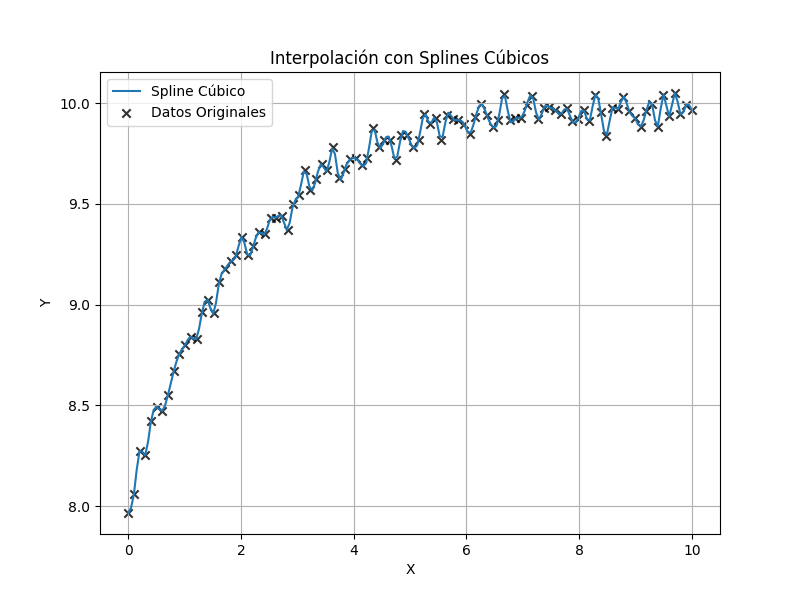
\includegraphics[width=0.6\textwidth]{img/interpolación splines.png}
    \caption{Interpolación con Splines Cúbicos aplicada a los datos experimentales.}
    \label{fig:spline}
\end{figure}

Los resultados muestran que los Splines Cúbicos \textbf{evitan las oscilaciones de alto grado} en los extremos y permiten un \textbf{ajuste más estable} a lo largo del dominio. 

Para analizar en detalle el comportamiento del Spline Cúbico, se observa lo siguiente en \textbf{diferentes regiones} del intervalo (véase la Figura~\ref{fig:splinesec}):

\begin{figure}[h]
    \centering
    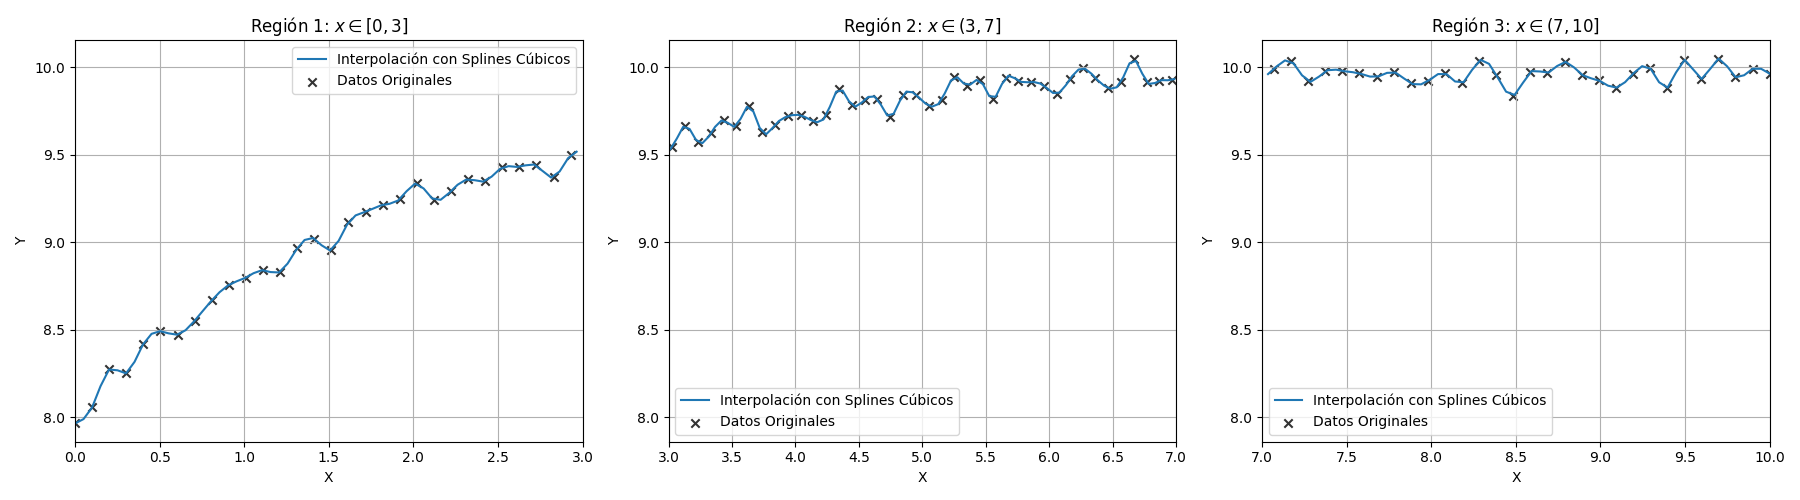
\includegraphics[width=0.9\textwidth]{img/spline_secciones.png}
    \caption{Análisis por Regiones de la Interpolación mediante Splines Cúbicos.}
    \label{fig:splinesec}
\end{figure}

\begin{itemize}
    \item \textbf{Región 1: $x \in [0,3]$.} La interpolación con Splines Cúbicos presenta un \textbf{ajuste preciso y suave} a los datos originales. La continuidad en la primera y segunda derivada garantiza una transición uniforme entre segmentos, evitando oscilaciones indeseadas. La baja dispersión en los puntos de datos y su disposición equiespaciada favorecen la estabilidad de la interpolación, asegurando una representación fiel de la tendencia general.

    \item \textbf{Región 2: $x \in (3,7]$.}  Se mantiene una \textbf{aproximación estable}, pero se observan \textbf{pequeñas variaciones} en torno a los valores originales. Estas fluctuaciones no corresponden a oscilaciones descontroladas, sino a la flexibilidad inherente del spline para adaptarse a los cambios locales sin comprometer la suavidad global. 

    \item \textbf{Región 3: $x \in (7,10]$.}  
    La interpolación sigue la distribución de los datos \textbf{sin introducir el Fenómeno de Runge}. El Spline Cúbico minimiza los errores de interpolación al fragmentar el dominio en intervalos locales. La estabilidad numérica se mantiene, y la precisión en los valores interpolados es mayor debido a la restricción de continuidad en las derivadas. Esto demuestra que los Splines Cúbicos son una alternativa eficiente y robusta para la interpolación en conjuntos de datos densos o con variabilidad localizada.
\end{itemize}

Los resultados confirman que la interpolación con Splines Cúbicos proporciona un ajuste más estable en comparación con la interpolación de Lagrange, especialmente en los extremos del intervalo. En la sección de \textbf{Discusión} (véase Sección~\ref{subsec:dsplines}), se compararán ambas técnicas en términos de estabilidad, precisión y aplicabilidad en distintos contextos.

\newpage
\subsection{Ejercicio 3: Ajuste por Regresión Lineal.}
Se han obtenido dos tipos de ajuste para los datos experimentales: mediante una \textbf{regresión polinómica de distintos grados} (1, 2, 3 y 4) utilizando el método de mínimos cuadrados, así como un ajuste utilizando una \textbf{función potencial} en una escala log-log: $y = a_0 x^{a_1}$. A partir de las gráficas obtenidas, se pueden extraer las siguientes observaciones clave:

\subsubsection*{Regresión polinómica.}
La Figura~\ref{fig:polinomios} muestra los resultados obtenidos para los distintos grados polinomiales en comparación con los datos originales.

\begin{figure}[h]
    \centering
    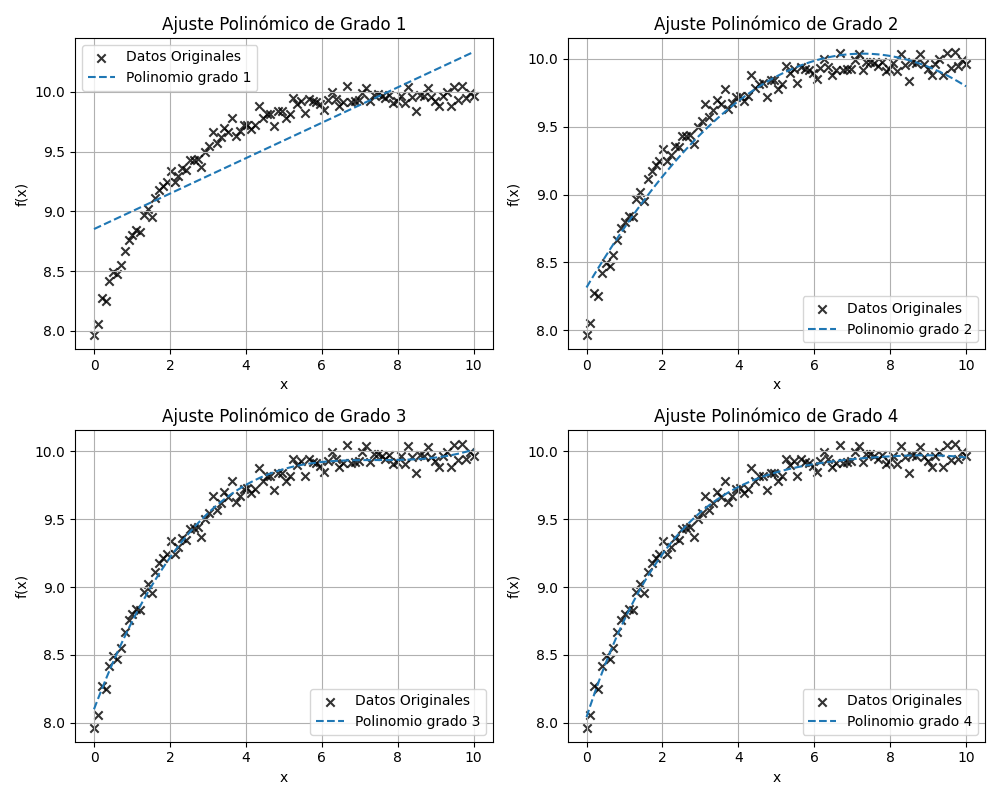
\includegraphics[width=0.7\linewidth]{img/polinomios_manual.png}
    \caption{Ajuste de los datos mediante regresión polinómica de distintos grados.}
    \label{fig:polinomios}
\end{figure}
\noindent Las ecuaciones de la rectas obtenidas y el coeficiente de determinación $R^2$ para cada ajuste polinómico se presentan en la Tabla~\ref{tab:ecuaciones_polinomios}.

\begin{table}[h]
    \centering
    \begin{tabular}{c|c|c}
        \hline
        \textbf{Grado} & \textbf{Ecuación del ajuste} & $R^2$ \\
        \hline
        1 & $y = 8.852 + 0.148x$ & $0.722340$ \\
        2 & $y = 8.316 + 0.472x - 0.032x^2$ & $0.958882$ \\
        3 & $y = 8.100 + 0.738x - 0.099x^2 + 0.004x^3$ & $0.987903$ \\
        4 & $y = 8.042 + 0.860x - 0.154x^2 + 0.013x^3 - 0.0004x^4$ & $0.989690$ \\
        \hline
    \end{tabular}
    \caption{Ecuaciones obtenidas y coeficiente de determinación $R^2$ para regresión polinómica.}
    \label{tab:ecuaciones_polinomios}
\end{table}

El ajuste por regresión polinómica muestra una mejora progresiva en la precisión conforme aumenta el grado del polinomio. 
\begin{itemize}
    \item \textbf{Polinomio de grado 1.} La ecuación obtenida ($y = 8.852 + 0.148x$) presenta un coeficiente de determinación $R^2 = 0.722$ lo que indica un \textbf{ajuste deficiente}. Este modelo lineal no logra capturar la curvatura de los datos, lo que resulta en una \textbf{subestimación sistemática} en los valores intermedios y una \textbf{sobreestimación} en los extremos.
    \item \textbf{Polinomio de grado 2.} El modelo cuadrático $y = 8.316 + 0.472x - 0.032x^2$ mejora significativamente la precisión, alcanzando un $R^2 = 0.959$. Este polinomio comienza a \textbf{capturar la curvatura} de la tendencia, proporcionando un \textbf{ajuste más preciso en la zona central}, aunque aún presenta \textbf{ciertas desviaciones} en los extremos del intervalo.
    \item \textbf{Polinomio de grado 3.} El ajuste mejora con el polinomio cúbico $y = 8.100 + 0.738x - 0.099x^2 + 0.004x^3$ que logra un $R^2 = 0.988$. Se observa que este modelo \textbf{ajusta con precisión} tanto la parte creciente como la estabilización de los datos en valores altos, reduciendo las desviaciones observadas en grados menores.
    \item \textbf{Polinomio de grado 4.} Este modelo $y = 8.042 + 0.860x - 0.154x^2 + 0.013x^3 - 0.0004x^4$ presenta el mejor ajuste con $R^2 = 0.99$.  Sin embargo, el \textbf{incremento en precisión respecto al modelo de grado 3 es marginal}, lo que sugiere que aumentar aún más el grado del polinomio podría no ser beneficioso y, en cambio, podría llevar a \textbf{sobreajuste}.
\end{itemize}
Estos resultados evidencian que los \textbf{modelos de grado bajo no son suficientes para capturar la estructura} de los datos, mientras que los \textbf{modelos de grado intermedio}, como el de grado 3, proporcionan un \textbf{equilibrio} adecuado entre precisión y estabilidad. Para analizar en mayor profundidad la implicación de estos resultados, se remite al apartado de \textbf{Discusión} (véase Sección~\ref{subsec:dregresion}).


\subsubsection*{Función potencial.}
La escala log-log $y = a_0 x^{a_1}$, revela relaciones de crecimiento lento y tendencias asintóticas. La Figura~\ref{fig:potencial} compara el ajuste de la función potencial con los datos originales.

\begin{figure}[h]
    \centering
    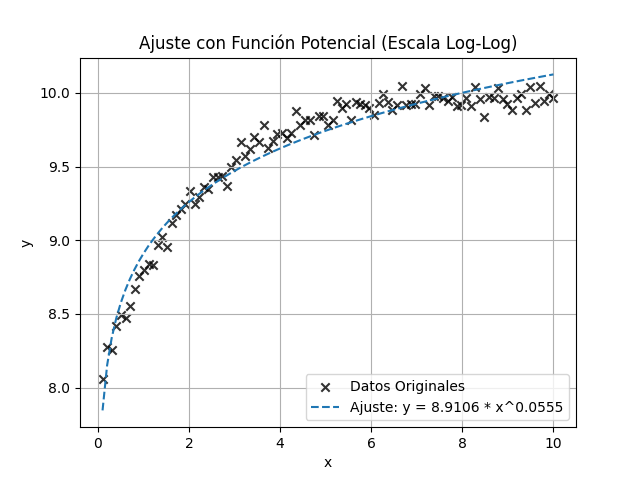
\includegraphics[width=0.6\linewidth]{img/funcion_potencial.png}
    \caption{Ajuste de los datos mediante función potencial.}
    \label{fig:potencial}
\end{figure}
\noindent El ajuste mediante una función potencial se realizó en una escala log-log, obteniendo la ecuación:
\begin{equation}
    y = 8.911 \cdot x^{0.056}
\end{equation}

En la \textbf{parte baja del dominio}, el modelo \textbf{captura} de manera efectiva la \textbf{curvatura inicial} de los datos, mostrando una buena concordancia con los valores originales. A medida que \textbf{$x$ aumenta}, la función de ajuste mantiene una \textbf{representación aceptable} de la tendencia general, aunque pueden observarse \textbf{pequeñas desviaciones} en los valores más altos. Sin embargo, la \textbf{forma global del ajuste es consistente con la estructura de los datos}, proporcionando una interpolación suavizada sin oscilaciones abruptas.\\

En términos de \textbf{precisión}, el modelo potencial presenta un coeficiente de determinación de $R^2=0.9547$, lo que indica un buen nivel de ajuste, aunque inferior a los obtenidos con \textbf{polinomios de grado 3 y 4}. \\

Para evaluar la idoneidad de este modelo, es relevante compararlo con la regresión polinómica vista previamente. Esta comparación se abordará en la \textbf{Discusión} (véase Sección~\ref{subsec:dregresion}).


\subsection{Ejercicio 4: Ajuste por Regresión No Lineal.}
Se realizó un ajuste a los datos experimentales utilizando distintos modelos de regresión no lineal, evaluando su desempeño en la aproximación de la relación entre las variables. Los modelos considerados fueron:

\begin{itemize}
    \item \textbf{Modelo Exponencial:} $f(x) = a_0 - a_1 e^{-a_2 x}$.
    \item \textbf{Modelo Lineal-Exponencial:} $f(x) = a_0 x - a_1 e^{-a_2 x}$.
    \item \textbf{Modelo Cuadrático-Exponencial:} $f(x) = a_0 x^2 - a_1 e^{-a_2 x}$.
\end{itemize}
La Figura~\ref{fig:nolineal} muestra la comparación entre los datos originales y los ajustes obtenidos con cada modelo.

\begin{figure}[h]
    \centering
    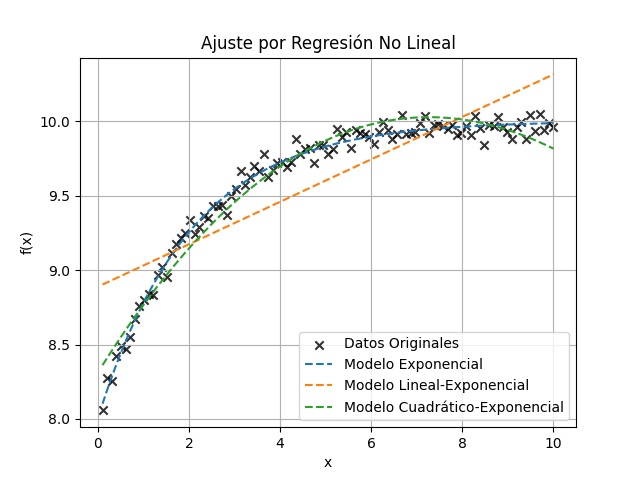
\includegraphics[width=0.6\linewidth]{img/regresion_no_lineal.png}
    \caption{Ajuste de los datos mediante modelos de regresión no lineal.}
    \label{fig:nolineal}
\end{figure}
\newpage
\noindent Los coeficientes de ajuste obtenidos para cada modelo, junto con sus valores de $R^2$, se presentan en la Tabla~\ref{tab:nolineal}.

\begin{table}[h]
    \centering
    \begin{tabular}{c|c|c|c|c|c}
        \hline
        \textbf{Modelo} & $a_0$ & $a_1$ & $a_2$ & $R^2$ & \textbf{Ecuación}\\
        \hline
        Exponencial & $10.0019$ & $1.9965$ & $0.4918$ & $0.991$ & $y = 10.0019 - 1.9965 e^{-0.4918x}$ \\
        Lineal-Exponencial & 0.1426 & $-8.8885$ & $-0.000003$ & $0.724$ & $y = 0.1426x - 8.8885 e^{-0.000003x}$ \\
        Cuadrático-Exponencial & $-0.0518$ & $-8.3125$ & $-0.0590$ & $0.965$ & $y = -0.0518x^2 - 8.3125 e^{-0.0590x}$ \\
        \hline
    \end{tabular}
    \caption{Coeficientes obtenidos y coeficiente de determinación $R^2$ para regresión no lineal.}
    \label{tab:nolineal}
\end{table}
\noindent De los resultados obtenidos se sacan las siguientes conclusiones:
\begin{itemize}
    \item \textbf{Modelo exponencial:} Representa un crecimiento que se desacelera a medida que $x$ aumenta, capturando adecuadamente la tendencia general de los datos en la parte inicial del intervalo. Sin embargo, en la región superior, el modelo muestra un error creciente para valores altos de $x$, lo que sugiere que su capacidad de predicción es más limitada en estos casos. A pesar de ello, su alto $R^2$ indica que sigue siendo el modelo más preciso en términos generales.

    \item \textbf{Modelo lineal-exponencial:} Presenta un ajuste menos preciso en comparación con los demás modelos, con un $R^2$ considerablemente menor. En la zona intermedia del intervalo, la pendiente lineal no logra capturar correctamente la curvatura de los datos, lo que lleva a \textbf{desviaciones significativas} en la predicción. Además, la \textbf{contribución del término exponencial} es mínima, haciendo que el modelo se comporte casi como una \textbf{regresión lineal simple} y perdiendo su capacidad de representar correctamente la tendencia de los datos.

    \item \textbf{Modelo cuadrático-exponencial:} Es el que mejor se ajusta a los datos a lo largo de todo el intervalo, manteniendo una buena correspondencia con la tendencia original. Su $R^2$ es alto, aunque ligeramente inferior al del modelo exponencial puro. La inclusión del término cuadrático permite capturar mejor la curvatura de los datos en la región inicial, reduciendo el error en comparación con los otros modelos. Sin embargo, en valores altos de $x$, su precisión no mejora significativamente con respecto al modelo exponencial.
\end{itemize}

Los resultados indican que, aunque el \textbf{modelo exponencial} es el \textbf{más preciso} en términos de $R^2$, el \textbf{modelo cuadrático-exponencial} ofrece un \textbf{compromiso razonable}, logrando una representación \textbf{equilibrada} en todas las regiones del intervalo. Para comprender mejor las diferencias entre estos modelos y su aplicabilidad, se realiza un análisis comparativo en el apartado de \textbf{Discusión}(véase Sección~\ref{subsec:rnolineal}).

%DISCUSIÓN
\newpage
\section{Discusión.}
\subsection{Ejercicio 1: Interpolación de Lagrange.}
\label{subsec:dlagrange}
La interpolación de Lagrange es \textbf{precisa en intervalos pequeños} con puntos distribuidos de manera uniforme, pero su \textbf{estabilidad disminuye conforme aumenta el número de nodos} o la densidad de datos. En particular, la última región mostrada en el apartado de \textbf{Resultados} (véase Sección~\ref{subsec:rlagrange}), mostró que los polinomios de alto grado tienden a oscilar en los extremos del intervalo, reduciendo la confiabilidad de la aproximación.

\subsubsection*{Eficiencia computacional.}
Desde el punto de vista \textbf{computacional}, la interpolación de Lagrange presenta una complejidad de $O(n^2)$ en la construcción del polinomio y $O(n)$ en su evaluación, ya que requiere evaluar productos de múltiples términos. Esto provoca que para \textbf{conjuntos de datos grandes, sea computacionalmente costoso}. Métodos alternativos, tales como los \textbf{Splines Cúbicos} (véase Sección~\ref{subsec:splines-cubicos}), ofrecen mayor eficiencia al dividir el dominio en segmentos, reduciendo el número de operaciones necesarias

\subsubsection*{Precisión y capacidad de ajuste.}
En términos de \textbf{precisión}, Lagrange es exacto en los nodos de interpolación, pero propenso a \textbf{errores en regiones con alta variabilidad} o con datos no equiespaciados. Por el contrario, los S\textbf{plines Cúbicos suavizan la interpolación} sin forzar un ajuste exacto, reduciendo oscilaciones y mejorando la representación global de los datos.

\subsubsection*{Estabilidad numérica y robustez.}
En cuanto a \textbf{estabilidad}, los \textbf{polinomios de alto grado son sensibles a pequeñas perturbaciones} en los datos, lo que puede generar \textbf{oscilaciones no deseadas}. Métodos como la \textbf{interpolación de Newton} (véase Sección~\ref{subsec:newton}) y los \textbf{Splines Cúbicos} distribuyen mejor los errores y evitan el crecimiento descontrolado del polinomio, lo que los hace más adecuados para aplicaciones prácticas que requieren robustez en la aproximación.

\subsection{Ejercicio 2: Interpolación mediante Splines Cúbicos.}
\label{subsec:dsplines}
Los Splines Cúbicos destacan por su capacidad para \textbf{generar interpolaciones suaves y estables}, lo que los convierte en una opción óptima en problemas dónde la \textbf{continuidad en las derivadas es crucial}. Su formulación basada en polinomios por tramos evita los inconvenientes de los polinomios de alto grado, distribuyendo la interpolación de manera más controlada y evitando oscilaciones innecesarias.\\

El \textbf{análisis comparativo} con la interpolación de \textbf{Lagrange} demuestra que los \textbf{Splines Cúbicos} son una opción más estable y eficiente en \textbf{escenarios con alta densidad} de puntos. Mientras que el polinomio de Lagrange puede generar oscilaciones en los extremos del intervalo, el Spline Cúbico evita estos problemas al dividir el dominio en segmentos locales.

\subsubsection*{Eficiencia computacional.}
Desde una perspectiva \textbf{computacional}, la eficiencia de los \textbf{Splines Cúbicos} es notable. La necesidad de resolver un sistema tridiagonal de ecuaciones lineales implica una complejidad de $O(n)$, lo que resulta más eficiente en comparación con el $O(n^2)$ de la \textbf{interpolación de Lagrange} (véase Sección~\ref{subsec:lagrange}). Esto los hace adecuados para conjuntos de datos grandes, dónde la velocidad de cálculo y la estabilidad numérica son factores determinantes.

\subsubsection*{Precisión y capacidad de ajuste.}
En términos de \textbf{precisión}, los \textbf{Splines Cúbicos} logran un \textbf{ajuste exacto} en los nodos de interpolación sin incurrir en sobreajustes globales. A diferencia de métodos que utilizan un único polinomio de alto grado, los Splines aseguran que la interpolación siga fielmente la tendencia de los datos sin introducir oscilaciones artificiales. En particular, su capacidad para conservar la continuidad en la primera y segunda derivada permite que la interpolación sea más natural y representativa en aplicaciones dónde la suavidad es un requisito clave.

\subsubsection*{Estabilidad numérica y robustez.}
En cuanto a \textbf{estabilidad}, los \textbf{Splines Cúbicos} son una alternativa robusta frente a otras metodologías de interpolación, ya que e\textbf{vitan la amplificación de errores} en los extremos y permiten un \textbf{control} más refinado de la curvatura de la función interpolada. Esto es especialmente relevante en problemas dónde los datos presentan variaciones localizadas, ya que la interpolación segmentada minimiza los errores acumulativos y mantiene la coherencia en la aproximación.

\subsubsection*{Comparación con la interpolación de Lagrange.}
Comparando con la \textbf{interpolación de Lagrange}, los resultados obtenidos confirman que los \textbf{Splines Cúbicos} son preferibles en situaciones dónde la \textbf{estabilidad} y la \textbf{eficiencia computacional} son \textbf{prioritarias}. Mientras que \textbf{Lagrange} puede generar oscilaciones indeseadas en regiones con alta densidad de puntos, los splines cúbicos logran un ajuste más controlado y menos susceptible a fluctuaciones. En consecuencia, su uso es recomendable en aplicaciones dónde la interpolación debe \textbf{preservar la suavidad y garantizar precisión en intervalos amplios} sin comprometer la estabilidad numérica (véase la Figura~\ref{fig:comparaar}).  

\begin{figure}[h]  
    \centering  
    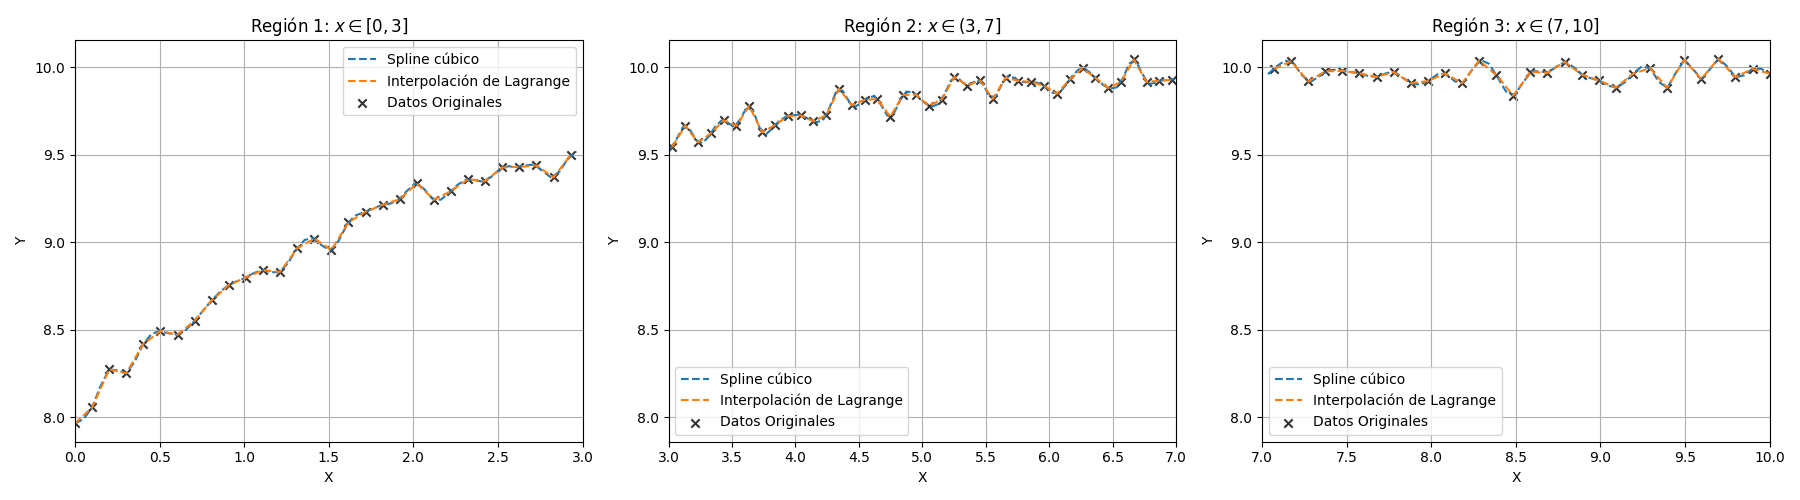
\includegraphics[width=0.9\linewidth]{img/comparacion.png}  
    \caption{Comparación por regiones: Interpolación de Lagrange y Splines Cúbicos.}
    \label{fig:comparaar}  
\end{figure} 

\newpage
\subsection{Ejercicio 3: Ajuste por Regresión Lineal.}
\label{subsec:dregresion}
\subsubsection*{Regresión polinómica.}
\begin{itemize}
    \item \textbf{Relación entre el grado del polinomio y la precisión del ajuste:} El \textbf{coeficiente de determinación} muestra un \textbf{aumento} progresivo a medida que el \textbf{grado del polinomio crece}, lo que indica que modelos de mayor orden pueden representar mejor la variabilidad de los datos. Sin embargo, la mejora entre los grados 3 y 4 es mínima, lo que sugiere que el \textbf{modelo de grado 3 es suficiente} para capturar la tendencia sin incurrir en complejidad innecesaria.
    \item \textbf{Sobreajuste y estabilidad del modelo:} Aumentar excesivamente el grado del polinomio puede llevar a un problema de sobreajuste, donde el modelo se ajusta demasiado a los datos de entrenamiento y pierde capacidad de generalización. Aunque el polinomio de grado 4 presenta un ajuste superior, su complejidad adicional podría no justificar el pequeño incremento en $R^2$. En aplicaciones prácticas, se recomienda optar por \textbf{modelos de grado intermedio para evitar oscilaciones}.
    \item  \textbf{Interpretabilidad y simplicidad del modelo:} Los \textbf{polinomios de grado bajo}, proporcionan una \textbf{interpretación más sencilla} de la relación entre las variables, pero \textbf{no capturan la curvatura de los datos}. A medida que aumenta el grado, el modelo se vuelve más flexible, pero también más difícil de interpretar. Se debe de encontrar un equilibrio entre precisión y simplicidad.
    \item \textbf{Eficiencia computacional:} Desde el punto de vista computacional, la regresión polinómica requiere resolver un sistema de ecuaciones normales, cuya \textbf{complejidad depende del grado del polinomio} y del método de solución utilizado. Para grados bajos, el cálculo es rápido y eficiente, pero a medida que el grado aumenta, los cálculos pueden volverse más costosos y propensos a inestabilidad numérica.


\end{itemize}

\subsubsection*{Función potencial.}
\begin{itemize}
    \item \textbf{Crecimiento desacelerado:} La ecuación obtenida indica que la variable dependiente crece con $x$, pero a un ritmo decreciente, lo que sugiere una \textbf{convergencia progresiva en valores altos de $x$}.
    \item \textbf{Escala log-log:} La transformación logarítmica utilizada en este ajuste permite \textbf{identificar patrones de crecimiento lento} o \textbf{comportamiento asintótico} en los datos. Esto es útil cuando se sospecha que la relación entre variables sigue una ley de potencias en lugar de una función polinómica.
    \item \textbf{Capacidad predictiva:} Si el objetivo es modelar tendencias generales y extrapolar datos fuera del intervalo analizado, el ajuste con función potencia es una opción adecuada, ya que mantiene estabilidad en la representación de los datos sin introducir fluctuaciones artificiales.
    \item \textbf{Eficiencia computacional:} El ajuste potencia requiere únicamente una regresión lineal en la escala log-log, lo que reduce su complejidad computacional a $O(n)$. Esto lo hace \textbf{Más eficiente que los polinomios de alto grado}, cuya solución requiere cálculos más costosos.
\end{itemize}
\subsubsection*{Comparación de Ajustes.}
\begin{itemize}
    \item \textbf{Precisión vs. estabilidad:} La regresión polinómica ofrece un ajuste más preciso dentro del intervalo de datos, alcanzando valores de $R^2$ superiores al ajuste potencial. Sin embargo, los \textbf{polinomios de grado alto pueden generar sobreajuste}, capturando ruido en los datos en lugar de representar la tendencia general. En cambio, la \textbf{función potencial} proporciona un ajuste más \textbf{estable} y \textbf{sin oscilaciones} indeseadas.
    \item \textbf{Extrapolación y generalización:} Si el propósito es simplemente \textbf{interpolar} dentro del conjunto de datos, \textbf{un polinomio} de grado intermedio o alto puede ser adecuado. No obstante, si se requiere \textbf{extrapolar}, la \textbf{función potencial es una opción más confiable}, ya que sigue una tendencia más predecible sin las oscilaciones que pueden aparecer en polinomios de alto grado.
    \item \textbf{Eficiencia computacional:} Mientras que los \textbf{polinomios} requieren la resolución de sistemas de ecuaciones de mayor complejidad $O(n^3)$ en su versión estándar, la \textbf{función potencial} reduce el problema a una regresión lineal en escala log-log, lo que implica menor costo computacional y una mayor estabilidad numérica.
\end{itemize}

\subsection{Ejercicio 4: Ajuste por Regresión No Lineal.}
\label{subsec:dnoregresion}
\subsubsection*{Comparación entre los modelos.}
\begin{itemize}
    \item \textbf{Precisión vs. estabilidad:} El \textbf{modelo exponencial} es el que presenta el \textbf{mayor $R^2$}, lo que indica que proporciona la \textbf{mejor precisión} dentro del intervalo de datos. Sin embargo, su \textbf{desviación en valores altos} de $x$ puede ser un \textbf{inconveniente} si se requiere una \textbf{representación uniforme} en todo el dominio. El modelo \textbf{cuadrático-exponencial}, aunque con un $R^2$ ligeramente menor, logra una \textbf{mejor estabilidad en el ajuste}, lo que lo hace más adecuado en escenarios donde se busca una \textbf{interpolación más homogénea}.
    
    \item \textbf{Eficiencia del modelo lineal-exponencial:} La baja precisión de este modelo sugiere que la \textbf{combinación de términos lineales y exponenciales no es efectiva} en este caso. La contribución del término exponencial es prácticamente despreciable, lo que hace que el modelo actúe como una regresión lineal simple sin capturar la curvatura real de los datos.

    \item \textbf{Capacidad de extrapolación:} En aplicaciones donde se requiera extrapolar datos más allá del intervalo analizado, la selección del modelo adecuado es crucial. Si bien el modelo exponencial captura bien la tendencia inicial, su error creciente en valores altos puede limitar su uso en predicciones a largo plazo. El \textbf{modelo cuadrático-exponencial podría ofrecer un mejor ajuste} en estas condiciones, aunque su estructura más compleja puede hacer que la extrapolación sea menos intuitiva.
\end{itemize}

\subsubsection*{Aplicabilidad y selección del modelo adecuado.}
\begin{itemize}
    \item Si se busca \textbf{máxima precisión} en la interpolación dentro del intervalo de datos, el \textbf{modelo exponencial} es la mejor opción.
    \item Si se \textbf{prioriza la estabilidad} del ajuste en todo el dominio, el \textbf{modelo cuadrático-exponencial} puede ser más adecuado.
    \item El \textbf{modelo lineal-exponencial es el menos recomendable}, ya que no captura correctamente la estructura de los datos.
\end{itemize}

Desde una perspectiva práctica, la elección del modelo \textbf{depende del propósito del análisis}. Para describir relaciones que sigan un comportamiento de crecimiento desacelerado, el modelo exponencial es una opción sólida. Sin embargo, si se requiere una mejor estabilidad en toda la región de análisis, el modelo cuadrático-exponencial puede proporcionar un mejor equilibrio entre precisión y generalización.

\newpage
\section{Conclusiones.}

La \textbf{interpolación de Lagrange} es precisa en regiones con puntos bien distribuidos, pero sufre inestabilidad en los extremos debido al \textbf{Fenómeno de Runge}, lo que la hace \textbf{poco recomendable para intervalos amplios}. Su alto costo computacional limita su uso en grandes volúmenes de datos.  \\


Los \textbf{Splines Cúbicos} ofrecen una alternativa más estable y eficiente a la \textbf{interpolación de Lagrange}, garantizando suavidad y continuidad sin oscilaciones no deseadas. Son ideales para interpolaciones donde se requiere estabilidad en todo el intervalo y menor complejidad computacional.   \\

La \textbf{regresión polinómica} de grado intermedio proporciona un \textbf{equilibrio} entre precisión y estabilidad, evitando el \textbf{sobreajuste} de polinomios de \textbf{grado alto}. Sin embargo, polinomios elevados pueden generar oscilaciones en la extrapolación y mayor costo computacional. El \textbf{ajuste con función potencial} es eficiente y adecuado para datos con crecimiento desacelerado. Aunque su precisión es menor que la polinómica, \textbf{evita oscilaciones extremas} y permite una extrapolación más estable con menor costo computacional.   \\

En la \textbf{regresión no lineal}, el \textbf{modelo exponencial} logra el mejor ajuste, aunque con errores crecientes en valores altos de $x$. El \textbf{modelo cuadrático-exponencial} mejora la estabilidad sin superar la precisión del exponencial puro, mientras que el \textbf{modelo lineal-exponencial} no logra captar la curvatura de los datos.   \\

En términos generales, para \textbf{interpolaciones precisas} dentro del intervalo, los \textbf{Splines Cúbicos} y los \textbf{polinomios de grado intermedio} son ideales. Para \textbf{estabilidad y extrapolación}, la \textbf{función potencia} y el \textbf{modelo exponencial} son mejores opciones. En términos de eficiencia, los \textbf{Splines Cúbicos} y la \textbf{función potencia} destacan sobre métodos de mayor complejidad.

%REFERENCIAS
\newpage
\section{Referencias.}
\renewcommand{\refname}{}
\renewcommand{\bibname}{}
\vspace{-10mm}
\begin{thebibliography}{99}

% Lagrange
\bibitem{lagrange1} Ingeniería UNAM. (s.f.). \textit{Interpolación de Lagrange}. Recuperado de \url{https://www.ingenieria.unam.mx/pinilla/PE105117/pdfs/tema4/4-1_lagrange.pdf}
\bibitem{lagrange2} Díaz, J. (s.f.). \textit{Interpolación de Lagrange}. Universitat de València. Recuperado de \url{https://www.uv.es/diazj/cn_tema5.pdf}
\bibitem{lagrange3} ANIEI. (s.f.). \textit{Curso de Métodos Numéricos}. Recuperado de \url{https://aniei.org.mx/paginas/uam/CursoMN/curso_mn_07.html}

% Splines Cúbicos
\bibitem{splines1} Díaz, J. (s.f.). \textit{Splines Cúbicos}. Universitat de València. Recuperado de \url{https://www.uv.es/diaz/mn/node40.html}
\bibitem{splines2} Universidad de Sevilla. (s.f.). \textit{Interpolación por Splines}. Recuperado de \url{https://biblus.us.es/bibing/proyectos/abreproy/3989/fichero/MEMORIA%252F13_ANEXO7.pdf}
\bibitem{splines3} UNAM. (s.f.). \textit{Métodos Numéricos en Ingeniería}. Recuperado de \url{https://www.paginaspersonales.unam.mx/app/webroot/files/4676/Asignaturas/1457/Archivo1.3288.pdf}
\bibitem{splines4} Universitat de Barcelona. (s.f.). \textit{Interpolación por Splines}. Recuperado de \url{https://diposit.ub.edu/dspace/bitstream/2445/122512/2/memoria.pdf}

% Ajuste Polinómico
\bibitem{polinomico1} UNAM. (s.f.). \textit{Regresión Polinómica}. Recuperado de \url{https://www.ccg.unam.mx/~vinuesa/R4biosciences/docs/Tema9_regresion.html}
\bibitem{polinomico2} Universidad de Murcia. (s.f.). \textit{Regresión Polinómica y Cuadrados Mínimos}. Recuperado de \url{https://webs.um.es/mhcifre/apuntes/Capitulo4.pdf}
\bibitem{polinomico3} Díaz, J. (s.f.). \textit{Regresión Polinómica}. Universitat de València. Recuperado de \url{https://www.uv.es/~diazj/cn_tema7.pdf}
\bibitem{polinomico4} Universidad del País Vasco. (s.f.). \textit{Regresión Polinómica}. Recuperado de \url{http://www.sc.ehu.es/sbweb/fisica3/datos/regresion/regresion.html}
\bibitem{polinomico5} Universidad de Buenos Aires. (s.f.). \textit{Regresión Lineal por Cuadrados Mínimos}. Recuperado de \url{https://materias.df.uba.ar/mytda2020c2/files/2013/03/RegresionLinealPorCuadradosMinimos.pdf}

% Regresión No Lineal
\bibitem{nolineal1} Universidad de Zaragoza. (s.f.). \textit{Modelos de Regresión No Lineal}. Recuperado de \url{https://ocw.unizar.es/ocw/pluginfile.php/2991/course/section/908/Tema%208_Modelos%20de%20Regresi%C3%B3n%20No%20lineal.pdf}
\bibitem{nolineal2} Universidad de Alicante. (s.f.). \textit{Regresiones Lineales y No Lineales}. Recuperado de \url{https://rua.ua.es/dspace/bitstream/10045/16373/4/Microsoft%20Word%20-%204.REGRESIONES%20LINEALES%20Y%20NO%20LINEALES.pdf}
\end{thebibliography}


%ANEXOS
\newpage
\section{Anexos.}
El código fuente de estas implementaciones está disponible en el siguiente repositorio de GitHub:  
\href{https://github.com/mgonzalz/sn_talleres/blob/main/notebooks/informe-01__interp_regresion.ipynb}{\texttt{GitHub - mgonzalz/sn\_talleres}}.

\subsection{Inicialización.}
En esta sección, se define una función para leer los datos desde un archivo de texto (`.txt`) utilizando NumPy. Luego, los datos se representan en un gráfico de dispersión mediante Matplotlib.
\lstinputlisting[style=python, caption=Lectura y graficación de datos.]{python/inicio.py}

\subsection{Función de Interpolación de Lagrange.}
En esta sección, se implementa la interpolación de Lagrange, calculando la base \(L_i(x)\) y evaluando el polinomio interpolador.

\lstinputlisting[style=python, caption=Implementación de la Interpolación de Lagrange.]{python/lagrange.py}

\newpage
\subsection{Función de Interpolación mediante Splines Cúbicos.}
En esta sección, se implementa la interpolación por splines cúbicos naturales, construyendo los polinomios por tramos y resolviendo un sistema tridiagonal para los coeficientes.

\lstinputlisting[style=python, caption=Implementación de la Interpolación por Splines Cúbicos.]{python/splines.py}

\newpage
\subsection{Ajuste Polinómico por Mínimos Cuadrados.}
En esta sección, se implementa el ajuste de un polinomio mediante el método de mínimos cuadrados, utilizando la matriz de Vandermonde para la estimación de coeficientes y la resolución de ecuaciones normales.

\lstinputlisting[style=python, caption=Implementación del Ajuste Polinómico por Mínimos Cuadrados.]{python/ajuste-polinomio.py}

\subsection{Ajuste Logarítmico por Mínimos Cuadrados}
En esta sección, se implementa el ajuste de una función potencial mediante el método de mínimos cuadrados, utilizando una transformación logarítmica para convertir el modelo en una regresión lineal en la escala log-log.

\lstinputlisting[style=python, caption=Implementación del Ajuste Logarítmico por Mínimos Cuadrados.]{python/ajuste-log.py}

\newpage
\subsubsection{Ajuste No Lineal: Métodos Automático y Manual.}

Para ajustar modelos no lineales a los datos disponibles, se proponen dos enfoques:

\begin{itemize}
    \item \textbf{Método Automático con curve\_fit}: Se utiliza la función \texttt{curve\_fit} de SciPy, que aplica internamente optimización no lineal basada en mínimos cuadrados. Es una opción rápida y eficiente para ajustar modelos sin necesidad de derivadas analíticas.
    \item \textbf{Método Manual con Gauss-Newton}: Se implementa el ajuste mediante el método de Gauss-Newton, calculando explícitamente la matriz Jacobiana para mejorar la convergencia. Este enfoque es útil cuando se requiere un control más preciso sobre el ajuste.
\end{itemize}

Dado que los datos de \( y \) contienen ruido, es importante modificar el ajuste para garantizar una mejor convergencia y minimizar la influencia de valores atípicos. A continuación, se presentan ambas implementaciones:

\lstinputlisting[style=python, caption=Ajuste No Lineal Automático con curve\_fit.]{python/ajuste-no-lineal_aut.py}

\newpage
\lstinputlisting[style=python, caption=Ajuste No Lineal Manual con Gauss-Newton.]{python/ajuste-no-lineal_manual.py}


\end{document}
